% Generator: hand-authored TikZ schematic traced from the fixed source; curve and coordinates are illustrative.
% Source ID: src-dcc6a2c21c7b8e7b8f23f5188f34d7f542f94e40f4219b54cfb85a0d7004bc0f
% PDF SHA-256: 7fc0fd289fc486a0ae1c16a9ab5b4f0561830897df6e8897c50666f03d511913
% PDF page 1; printed page 126; question 5.
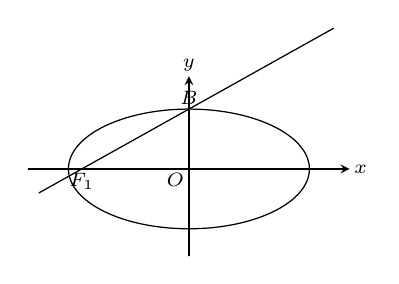
\begin{tikzpicture}[
  x=0.68cm,y=0.76cm,line width=0.45pt,line cap=round,>=stealth,
  every node/.style={font=\scriptsize,inner sep=1.5pt}
]
  \draw[->] (-3.0,0)--(3.0,0) node[right] {$x$};
  \draw[->] (0,-1.45)--(0,1.55) node[above] {$y$};
  \draw (0,0) ellipse [x radius=2.25,y radius=1.0];
  \draw (-2.8,-0.4)--(2.7,2.35);

  \node[below left] at (0,0) {$O$};
  \node[above] at (0,1) {$B$};
  \node[below] at (-2,0) {$F_1$};
\end{tikzpicture}
